\hypertarget{EXMPLE_8cpp}{}\section{/home/visxim/\+C\+Lion\+Projects/\+Configuration\+\_\+daemon/\+E\+X\+M\+P\+LE.cpp File Reference}
\label{EXMPLE_8cpp}\index{/home/visxim/\+C\+Lion\+Projects/\+Configuration\+\_\+daemon/\+E\+X\+M\+P\+L\+E.\+cpp@{/home/visxim/\+C\+Lion\+Projects/\+Configuration\+\_\+daemon/\+E\+X\+M\+P\+L\+E.\+cpp}}


\hyperlink{classEXMPLE}{E\+X\+M\+P\+LE} method definition.  


{\ttfamily \#include \char`\"{}E\+X\+M\+P\+L\+E.\+h\char`\"{}}\newline
Include dependency graph for E\+X\+M\+P\+L\+E.\+cpp\+:
\nopagebreak
\begin{figure}[H]
\begin{center}
\leavevmode
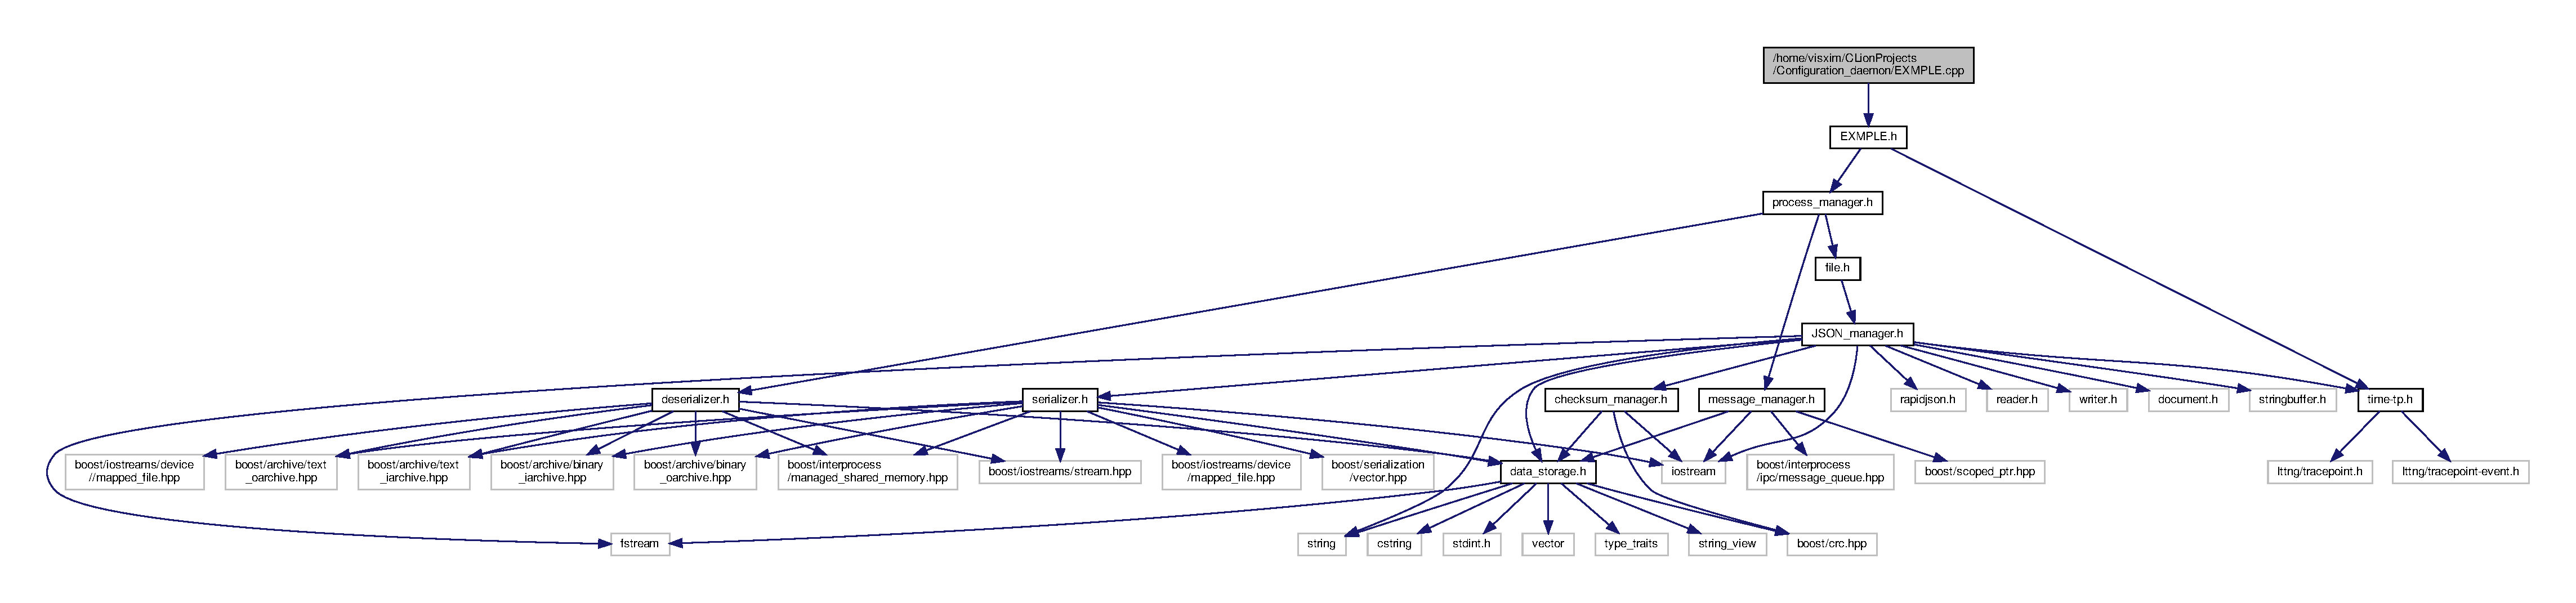
\includegraphics[width=350pt]{EXMPLE_8cpp__incl}
\end{center}
\end{figure}


\subsection{Detailed Description}
\hyperlink{classEXMPLE}{E\+X\+M\+P\+LE} method definition. 

The \hyperlink{classupdate__manager}{update\+\_\+manager} is derived from the \hyperlink{classprocess__manager}{process\+\_\+manager}, it is created to specifically configure the the \hyperlink{classupdate__manager}{update\+\_\+manager} process 